
\documentclass{beamer}

\newtheorem{conjecture}{Conjecture}
 \newcommand{\bconj}[1]{\begin{conj}#1\end{conj}}
\newtheorem{mconj}{Metaconjecture}

\newtheorem{prop}{Proposition}
 \newcommand{\bprop}[1]{\begin{prop}#1\end{prop}}
\newtheorem{lem}{Lemma}
 \newcommand{\blem}[1]{\begin{lem}#1\end{lem}}


\newtheorem{guess}{Guess}
 \newcommand{\bguess}[1]{\begin{guess}#1\end{guess}}
%\newtheorem{corollary}{Corollary}



\usepackage{tikz,framed, amsrefs, amsthm}
\tikzstyle{every node}=[circle, draw, fill=black!50,
                        inner sep=0pt, minimum width=4pt]
\tikzstyle{lblvertex}=[fill=white, inner sep = 1pt, font=\small]
\tikzstyle{lblvertex2}=[fill=white, inner sep = 1pt, font=\tiny,circle, draw]
\tikzstyle{lblvertex3}=[fill=white, inner sep = 1pt, font=\tiny,circle, draw = black!25]
\tikzstyle{words} =[rectangle, draw=none, fill=none, black]
\newcommand{\bframe}[2]{\begin{frame}{#1}#2\end{frame}}
\newcommand{\bfig}[2]{\begin{figure}#1\caption{#2}\end{figure}}


\usetheme{CambridgeUS}
\setbeamertemplate{navigation symbols}{}
\usecolortheme[RGB={216,30,5}]{structure}
\AtBeginSection[] % "Beamer, do the following at the start of every section"
{
\begin{frame}<beamer>
\frametitle{Outline} % make a frame titled "Outline"
\tableofcontents[currentsection] % show TOC and highlight current section
\end{frame}
}

\title{Connected matchings in special families of graphs}
\author{Chris Caragianis}
\institute[U of L]{ Department of Mathematics\\ University of Louisville\\ Louisville, KY 40292\\[1ex]
   \texttt{cjcara01@louisville.edu} }
\begin{document}

\bframe{}{\titlepage}

\bframe{}{\tableofcontents}

\section{Introduction}

\subsection{Review of graph-theoretic concepts}

\bframe{Graphs, vertex coloring}{
	\begin{overprint} 
		\onslide<1>A (simple, undirected) graph is comprised of a collection of \textit{vertices}, some pairs of which are \textit{adjacent}.  A pair of adjacent vertices is called an \textit{edge}. \\
		\onslide<2-3>A (simple, undirected) graph is comprised of a collection of \textit{vertices}, some pairs of which are \textit{adjacent}.  A pair of adjacent vertices is called an \textit{edge}. \vskip 0.5 cm A proper vertex coloring is one in which adjacent vertices recieve different colors.
	\end{overprint}	
	\vskip 1 cm 
		\only<1-2>{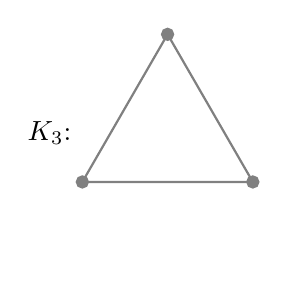
\begin{tikzpicture}[thick,scale=0.5]
\draw[gray] 
    {
		(180:3) node[words] {$K_3$:}
        (90:2.5) node {}  -- (210:2.5)
		(210:2.5) node {} -- (-30:2.5)
		(-30:2.5) node {} -- (90:2.5)
		(-90:3.5) node[words] {}
    };

\end{tikzpicture}
}\only<3>{\input{triangle_prop}} \qquad 
		\only<1-2>{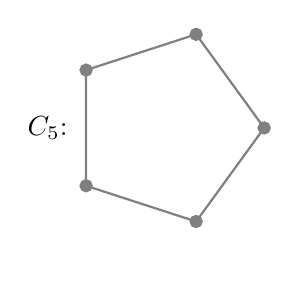
\begin{tikzpicture}[thick,scale=0.5]
\draw[gray] 
    {
		(180:3) node[words] {$C_5$:}
        (72:2.5) node {}  -- (144:2.5)
		(144:2.5) node {} -- (216:2.5)
		(216:2.5) node {} -- (288:2.5)
		(288:2.5) node {}  -- (0:2.5)
		(0:2.5) node {} -- (72:2.5)
		(-90:3.5) node[words] {}
    };
	
\end{tikzpicture}
}\only<3>{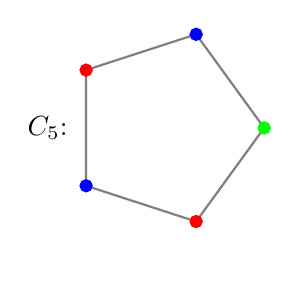
\begin{tikzpicture}[thick,scale=0.5]
\draw[gray] 
    {
		(180:3) node[words] {$C_5$:}
        (72:2.5) node[blue] {}  -- (144:2.5)
		(144:2.5) node[red] {} -- (216:2.5)
		(216:2.5) node[blue] {} -- (288:2.5)
		(288:2.5) node[red] {}  -- (0:2.5)
		(0:2.5) node[green] {} -- (72:2.5)
		(-90:3.5) node[words] {}
    };
	
\end{tikzpicture}
} \qquad 
		\only<1-2>{\begin{tikzpicture}[thick,scale=0.5]
\draw[gray] 
    {
		(180:3) node[words] {$G$:}
        (90:2.5) node {}  -- (0:0)
		(210:2.5) node {} -- (0:0)
		(-30:2.5) node {} -- (0:0)
		(0:0) node {}
		(-90:3.5) node[words] {}
    };

\end{tikzpicture}
}\only<3>{\begin{tikzpicture}[thick,scale=0.5]
\draw[gray] 
    {
		(180:3) node[words] {$G$:}
        (90:2.5) node[red] {}  -- (0:0)
		(210:2.5) node[red] {} -- (0:0)
		(-30:2.5) node[red] {} -- (0:0)
		(0:0) node[blue] {}
		(-90:3.5) node[words] {}
    };

\end{tikzpicture}
}}

\bframe{Clique number, independence number}{
	\begin{itemize}
		\item A \textit{clique} on $n$ vertices (also called a \textit{complete graph}) is a collection of $n$ vertices along with all possible edges.\pause  
		\item The \textit{clique number} of $G$, denoted $\omega(G)$, is the size of the largest clique in $G$.\pause  
		\item The \textit{independence number} of $G$, denoted $\alpha(G)$, is the size of the largest set of vertices from $G$ that induces no edges.\pause
	\end{itemize}
	\begin{center}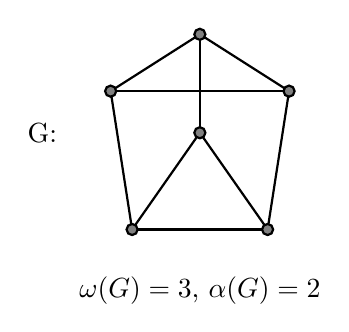
\begin{tikzpicture}[thick,scale=0.5]

	\coordinate (a) at (90:2.5);
	\coordinate (b) at (25:2.5); 
	\coordinate (c) at (0:0);
	\coordinate (d) at (155:2.5);
	\coordinate (e) at (-55:3);
	\coordinate (f) at (-125:3);

	\draw (a)--(b);
	%\draw (b)--(c);
	\draw (d)--(a);
	\draw (a)--(c);
	%\draw (c)--(d);
	\draw (b)--(e);
	\draw (e)--(c);
	\draw (d)--(f);
	\draw (f)--(c);
	\draw (d)--(b);
	\draw (e)--(f);
	%\draw (f) arc {-125:-33:3};
	
	\draw (a) node {};
	\draw (b) node {};
	\draw (c) node {};
	\draw (d) node {};
	\draw (e) node {};
	\draw (f) node {};
	\draw (-90:4) node[words] {$\omega(G) = 3$, $\alpha(G) = 2$};
	\draw (180:4) node[words] {G:};
\end{tikzpicture}
\end{center}}

\bframe{Chromatic number}{The \textit{chromatic number} of a graph $G$, denoted $\chi(G)$, is the minimum number of colors needed to properly color the vertices of $G$.
	\begin{overprint}	
		\onslide<1>\vskip 1 cm \input{triangle_prop} \qquad 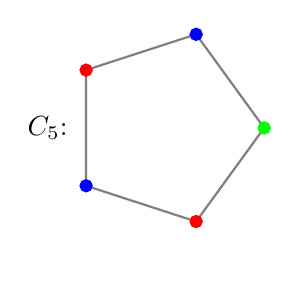
\begin{tikzpicture}[thick,scale=0.5]
\draw[gray] 
    {
		(180:3) node[words] {$C_5$:}
        (72:2.5) node[blue] {}  -- (144:2.5)
		(144:2.5) node[red] {} -- (216:2.5)
		(216:2.5) node[blue] {} -- (288:2.5)
		(288:2.5) node[red] {}  -- (0:2.5)
		(0:2.5) node[green] {} -- (72:2.5)
		(-90:3.5) node[words] {}
    };
	
\end{tikzpicture}
 \qquad \begin{tikzpicture}[thick,scale=0.5]
\draw[gray] 
    {
		(180:3) node[words] {$G$:}
        (90:2.5) node[red] {}  -- (0:0)
		(210:2.5) node[red] {} -- (0:0)
		(-30:2.5) node[red] {} -- (0:0)
		(0:0) node[blue] {}
		(-90:3.5) node[words] {}
    };

\end{tikzpicture}
\\
		\onslide<2>\vskip 1 cm \input{triangle_prop_chi} \qquad \input{c5_prop_chi} \qquad \input{claw_prop_chi}
	\end{overprint}}

\subsection{Connected matchings}

\bframe{Connected matchings}{
 A {\it matching} in a graph $G$ is a collection of disjoint edges. \pause\vskip 0.5 cm
 A \textit{connected matching} is a collection of disjoint edges such that each pair of edges has a pair of adjacent endpoints. \pause
	\begin{center}
	\begin{overprint}
		\onslide<3>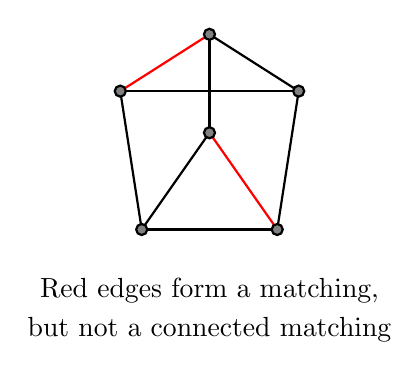
\begin{tikzpicture}[thick,scale=0.5]

	\coordinate (a) at (90:2.5);
	\coordinate (b) at (25:2.5); 
	\coordinate (c) at (0:0);
	\coordinate (d) at (155:2.5);
	\coordinate (e) at (-55:3);
	\coordinate (f) at (-125:3);

	\draw (a)--(b);
	%\draw (b)--(c);
	\draw[red] (d)--(a);
	\draw (a)--(c);
	%\draw (c)--(d);
	\draw (b)--(e);
	\draw[red] (e)--(c);
	\draw (d)--(f);
	\draw (f)--(c);
	\draw (d)--(b);
	\draw (e)--(f);
	%\draw (f) arc {-125:-33:3};
	
	\draw (a) node {};
	\draw (b) node {};
	\draw (c) node {};
	\draw (d) node {};
	\draw (e) node {};
	\draw (f) node {};
	\draw (-90:4) node[words] {Red edges form a matching,};
	\draw (-90:5) node[words] {but not a connected matching};
\end{tikzpicture}
\\
		\onslide<4-> 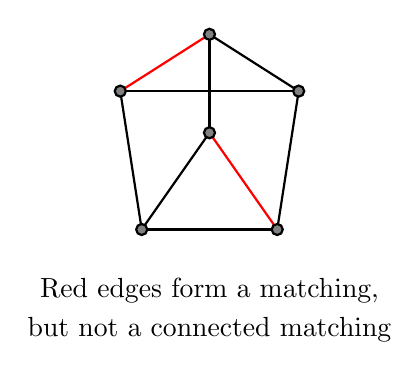
\begin{tikzpicture}[thick,scale=0.5]

	\coordinate (a) at (90:2.5);
	\coordinate (b) at (25:2.5); 
	\coordinate (c) at (0:0);
	\coordinate (d) at (155:2.5);
	\coordinate (e) at (-55:3);
	\coordinate (f) at (-125:3);

	\draw (a)--(b);
	%\draw (b)--(c);
	\draw[red] (d)--(a);
	\draw (a)--(c);
	%\draw (c)--(d);
	\draw (b)--(e);
	\draw[red] (e)--(c);
	\draw (d)--(f);
	\draw (f)--(c);
	\draw (d)--(b);
	\draw (e)--(f);
	%\draw (f) arc {-125:-33:3};
	
	\draw (a) node {};
	\draw (b) node {};
	\draw (c) node {};
	\draw (d) node {};
	\draw (e) node {};
	\draw (f) node {};
	\draw (-90:4) node[words] {Red edges form a matching,};
	\draw (-90:5) node[words] {but not a connected matching};
\end{tikzpicture}
\qquad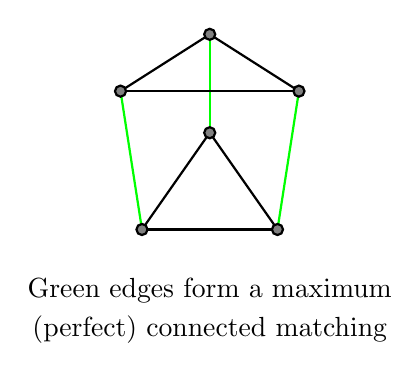
\begin{tikzpicture}[thick,scale=0.5]

	\coordinate (a) at (90:2.5);
	\coordinate (b) at (25:2.5); 
	\coordinate (c) at (0:0);
	\coordinate (d) at (155:2.5);
	\coordinate (e) at (-55:3);
	\coordinate (f) at (-125:3);

	\draw (a)--(b);
	%\draw (b)--(c);
	\draw (d)--(a);
	\draw[green] (a)--(c);
	%\draw (c)--(d);
	\draw[green] (b)--(e);
	\draw (e)--(c);
	\draw[green] (d)--(f);
	\draw (f)--(c);
	\draw (d)--(b);
	\draw (e)--(f);
	%\draw (f) arc {-125:-33:3};
	
	\draw (a) node {};
	\draw (b) node {};
	\draw (c) node {};
	\draw (d) node {};
	\draw (e) node {};
	\draw (f) node {};
	\draw (-90:4) node[words] {Green edges form a maximum};
	\draw (-90:5) node[words] {(perfect) connected matching};
\end{tikzpicture}

	\end{overprint}
	\end{center}\pause
We will denote by $\nu_c(G)$ the size of a maximum connected matching in $G$.
}

\bframe{Separable edges, Neighborly edges}{

If a pair of edges $e $ and $f$ from a graph $G$ are disjoint and have no pair of adjacent endpoints then we say that $e$ and $f$ are {\it separable}. \pause\vskip 0.5 cm

Otherwise, we say $e$ and $f$ are {\it neighborly}. \pause\vskip 0.5 cm
\begin{center}
	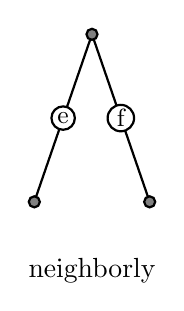
\begin{tikzpicture}[thick,scale=0.75]

	\coordinate (a0) at (0:0);
	\coordinate (a1) at (180:1);
	\coordinate (a3) at (-109:3);
	\coordinate (a2) at (0:1);
	\coordinate (a4) at (-71:3);
	\coordinate (text) at (-90:4);
	\coordinate (b2) at (30:3);

	\draw (a0)-- node[lblvertex] {e}(a3);
	\draw (a0)-- node[lblvertex] {f}(a4);

	\draw (a0) node {};	
	\draw (text) node[words] {neighborly};
	\draw (a3) node {};
	\draw (a4) node {};
	
\end{tikzpicture}
\qquad\pause
	\input{nonsep2}\qquad\pause
	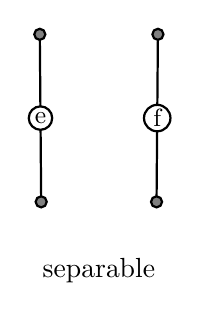
\begin{tikzpicture}[thick,scale=0.75]

	\coordinate (a0) at (0:0);
	\coordinate (a1) at (180:1);
	\coordinate (a3) at (-109:3);
	\coordinate (a2) at (0:1);
	\coordinate (a4) at (-71:3);
	\coordinate (b1) at (150:3);
	\coordinate (text) at (-90:4);

	\draw (a1)-- node[lblvertex] {e}(a3);
	\draw (a2)-- node[lblvertex] {f}(a4);
	\draw (a1) node[]{};
	\draw (a2) node[]{};
	\draw (a3) node[]{};
	\draw (a4) node[]{};
	\draw (text) node[words] {separable};
	
\end{tikzpicture}
 \pause
\end{center}
\vskip 0.5 cm
A graph that contains a separable pair of edges is called separable.  \pause A connected matching is a matching which contains no separable pair.

}


\section{Connected matchings and Hadwiger's conjecture}

\subsection{Hadwiger's conjecture}

\bframe{Perfect graphs}{
	For any graph $G$, $\chi(G) \geq \omega(G)$\pause, but the converse is not true.\pause
\begin{center}
 \input{c5_prop_chi} 
\end{center}
\pause

	We say that a graph $G$ is \textit{perfect} if for every induced subgraph $H$ of $G$, $\chi(H) = \omega(H)$.\pause 
\begin{theorem}[Strong perfect graph theorem (SPGT)]A graph $G$ is perfect if and only if for each $k >1$ it has neither a $C_{2k+1}$ nor its complement as an induced subgraph.\end{theorem}}

\bframe{Toft's ``metaconjecture''}{

Is there a structure in graphs the size of which provides an {\it upper } bound to the chromatic number?\pause\vskip 0.5 cm 

Bjarne Toft framed the question in this way \cite{MR1411244}: \pause
\begin{mconj}
The largest number of colors needed to color any graph in a topological class is precisely the largest number of vertices in any complete graph belonging to the class
\end{mconj}\pause\vskip 0.25 cm 
One way of defining ``topological class'' is using {\it graph minors}.
}


\bframe{Graph minors}{We say that a graph $G$ contains $H$ \textit{as a minor}, (denoted $G\geq H$), if $H$ is obtained from $G$ by successive vertex deletions and edge contractions.\pause \vskip 0.5 cm
An ``edge contraction'' consists of identifying two adjacent vertices, the resulting vertex being adjacent to any neighbors of either.\pause

\begin{center}
 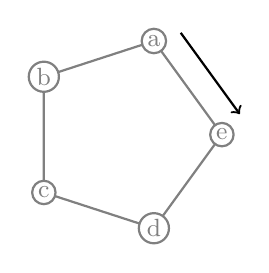
\begin{tikzpicture}[thick,scale=0.5]
\draw[gray] 
    {
        (72:2.5) node[lblvertex] {a}  -- (144:2.5)
		(144:2.5) node[lblvertex] {b} -- (216:2.5)
		(216:2.5) node[lblvertex] {c} -- (288:2.5)
		(288:2.5) node[lblvertex] {d}  -- (0:2.5)
		(0:2.5) node[lblvertex] {e} -- (72:2.5)
		
	
    };
	\draw (62:3)node[words] {}
		edge[->] (10:3);
	
\end{tikzpicture}
 \quad\pause
 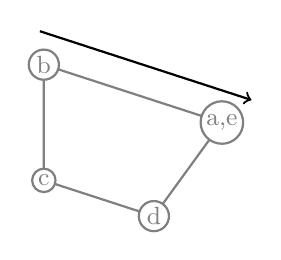
\begin{tikzpicture}[thick,scale=0.5]
\draw[gray] 
    {
        
		(144:2.5) node[lblvertex] {b} -- (216:2.5)
		(216:2.5) node[lblvertex] {c} -- (288:2.5)
		(288:2.5) node[lblvertex] {d}  -- (0:2.5)
		(0:2.5) node[lblvertex] {a,e} -- (144:2.5)
	
    };
	\draw (134:3.3)node[words] {}
		edge[->] (10:3.3);
	
\end{tikzpicture}
\quad\pause
 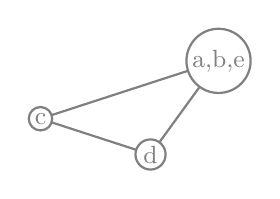
\begin{tikzpicture}[thick,scale=0.5]
\draw[gray] 
    {
        
		
		(216:2.5) node[lblvertex] {c} -- (288:2.5)
		(288:2.5) node[lblvertex] {d}  -- (0:2.5)
		(0:2.5) node[lblvertex] {a,b,e} -- (216:2.5)
	
    };
	
	
\end{tikzpicture}
\pause
\vskip 0.25 cm 
$C_5 \geq K_3$
\end{center}

	 }

\bframe{Hadwiger's conjecture}{
    It is widely believed, but is yet to be proved, that the size of the largest complete minor in a graph is an upper bound on the chromatic number. \pause
\vskip 0.5 cm Formally, let $\eta(G)$ be the largest $n$ for which $G \geq K_n$.\pause
 \vskip 0.5 cm \begin{conjecture}[Hadwiger, 1943] For all graphs $G$, \[\eta(G) \geq \chi(G)\] 
\end{conjecture}
 }

\subsection{A weaker conjecture than Hadwigers}

\bframe{A weaker conjecture.}{

	For all graphs $G$ on $n$ vertices, $n/\alpha(G) \leq \chi(G)$.\pause\vskip 0.5 cm
 The following conjecture is then implied by Hadwiger's.\pause
\begin{conjecture}\label{hc}
 For any graph $G$ on $n$ vertices with $\alpha(G) =\alpha$, \[\eta(G) \geq \frac{n}{\alpha}\]
\end{conjecture}
\pause \vskip 0.25 cm

Plummer, Stiebitz and Toft  show in \cite{MR2070161} that this is equivalent to Hadwiger's conjecture for graphs with independence number two.

}

\bframe{}{
 Duchet and Meyniel showed in  \cite{MR671905} (1982) that $\displaystyle\eta(G) \geq \frac{ n}{2\alpha - 1}$.\pause \vskip 0.5 cm 

When $\alpha \geq 3$, Kawarabayashi, Plummer and Toft \cite{MR2156345} improve this to 
\[\eta(G) \geq \frac{n(4\alpha-2)}{(4\alpha-3)(2\alpha -1)}\].   \pause  When $\alpha = 2$, the result of Duchet and Meyniel is still the best known. \pause \vskip 0.5 cm

The problem of reducing the constant of $1/3$ in the $\alpha  = 2 $ case remains. 
}

\subsection{Connected matchings in $\alpha = 2$ graphs}

\bframe{An extremal conjecture for connected matchings}{
  Gy\'arf\'as, F\"uredi and Simonyi observe this and conjecture \pause 
 	\begin{conjecture}[\cite{FGS}]
  		There exists an absolute constant $c$ so that any graph $G$ with $\alpha(G) =2$ and at least $ct$ vertices has a connected matching of at least $t$ edges.
 	\end{conjecture}\vskip 0.5 cm\pause
 	If true, this would imply that when $\alpha(G) = 2$, $\eta(G) > n/3$. \pause\vskip 0.5 cm 
 They further conjecture that $c = 4$ and prove this for $t \leq 17$.}

\bframe{Partial results}{

We have the following partial results toward resolving this conjecture.
\pause \vskip 0.5 cm
Fix $c < 1/4$ and let $G$ be a graph on $n$ vertices with $\alpha(G) = 2$ and no connected matching of size $cn$. \pause \vskip 0.25 cm
\begin{enumerate}
	\item $\omega(G) < cn$ \pause
	\item $G$ is $\displaystyle\left( \frac{c-1}{c}\right)n$ connected \pause
	\item For any constant $b$ and $n$ sufficiently large, $\omega(G) \geq b\sqrt{n\log n}$  
\end{enumerate}
}

\bframe{Proof of 1}{
\pause

Let $S$ be a set of $cn$ vertices inducung a clique. \pause For any subset of $S'\subseteq S$, the intersection $\displaystyle I_{S'} = \bigcap_{s\in S'} \{v \in V(G): sv \notin E(G)\}$ induces a clique. \pause If for any $S'\subseteq S$, $|I_{S'}| > n/2$, then there is a $cn$-connected matching in the clique induced by $I_{S'}$. 
}

\bframe{Proof of 1, continued} {Otherwise, $|N(S')| \geq |S'|$ for all $S'\subseteq S$, and there is an $S-(V(G)-S)$ matching saturating $S$. \pause This matching must be connected, since $S$ induces a clique.

}

\bframe{Proof of 2}{
\pause
First of all, note that from 1, we can assume $G$ is $n/2$ connected.  \pause
Let $S$ be a minimum cut set of $G$.  \pause We want to show that there is a connected matching saturating $V(G) - S$.\pause\vskip 0.5 cm 

Every vertex of $G$ is complete to $L$ or complete to $R$.  \pause We claim that between any $A \subseteq S_L$ (with $|A| \leq |R|$) and $R$, there is a matching saturating $A$. \pause 

}

\bframe{Proof of 2, continued}{

If there is no such matching, Hall's condition implies that there is $T \subseteq A$ such that $|N(T) \cap R| < T$.  \pause If this is the case, then $(S-T ) \cup (N(T) \cap R)$ is a cut set separating $L\cup T$ and $R-N(T)$. \pause This cut set is smaller than $S$, so we have a contradiction. \pause (This argument follows Blasiak \cite{blas})

}

\bframe{Proof of 2, continued}{

Now let $M$ be the largest matching obtained with $(S_L,R)$ edges and $(S_R,L)$ edges.  \pause 
This matching is connected, and $|M| = \min\{|S_L|, |R|\} + \min\{|S_R|, |L|\}$. \pause 
If both $|R| \leq S_L$ and $|L| \leq S_R$, then we are done.  
}

\bframe{Proof of 2, continued}{
If, WLOG,  $|R| > S_L$, then let $U_R$ denote the set of vertices of $R$ unmatched by $M$. \pause
 Since $|S|\geq n/2$, there are at least $|U_R|$ unmatched vertices of $S_R$ (denoted $U_{S_R}$).\pause
  Augment $M$ with any $(U_R , U_{S_R})$ matching saturating $U_R$ to yield $M'$. \pause
 Hence, $M'$ is a $(S,S^c)$ connected matching saturating $S^c = R\cup L$, and $|R\cup L| = n-\kappa(G)$. 
}

\bframe{}{
We will delay the proof of 3 until introducing some useful notation.
}

\section{Proximity Partitions}

\subsection{Basic facts and definitions}

\bframe{Definition}{
	Given a graph $G$ on $n$ vertices, we define the \textit{proximity $k$-partition} $\mathcal{P} = \{P_1, P_2, \ldots, P_k\}$ of the edges of $K_n$ induced by $G$ as follows.\pause\vskip 0.5 cm

	For all $u,v \in V(G)$, $i < k$
 	\begin{enumerate}
  		\item $uv \in P_i$ if and only if $d_G(u,v) = i$\pause
  		\item $uv \in P_k$ if and only if $d_G(u,v) \geq k$\pause
 	\end{enumerate}
	\vskip 0.5 cm
	\begin{center}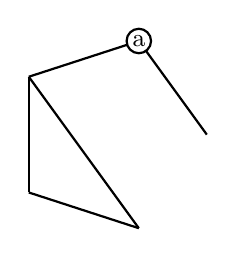
\begin{tikzpicture}[thick,scale=0.5]

	\coordinate (a1) at (72:2.5);
	\coordinate (a2) at (144:2.5); 
	\coordinate (a3) at (216:2.5);
	\coordinate (a4) at (288:2.5);
	\coordinate (a5) at (0:2.5);

	\draw (a5)--(a1);
	\draw (a1)--(a2);
	\draw (a2)--(a3);
	\draw (a2)--(a4);
	\draw (a3)--(a4);

	\draw (a1) node[lblvertex] {a};  
	
\end{tikzpicture}
\pause\quad 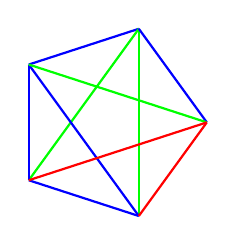
\begin{tikzpicture}[thick,scale=0.5]

	\coordinate (a1) at (72:2.5);
	\coordinate (a2) at (144:2.5); 
	\coordinate (a3) at (216:2.5);
	\coordinate (a4) at (288:2.5);
	\coordinate (a5) at (0:2.5);
	
	\draw[blue] (a1)--(a2);	
	\draw[green,] (a1)-- (a3);
	\draw[green] (a1)--(a4);
	\draw[blue] (a1)--(a5);
	\draw[blue] (a2)--(a3);	
	\draw[blue] (a2)--(a4);	
	\draw[green] (a2)--(a5);
	\draw[blue] (a3)--(a4);
	\draw[red] (a3)--(a5);
	\draw[red] (a4)--(a5);
	
	
\end{tikzpicture}
\end{center}}

\bframe{Proximity colorings}{
	We will be primarily interested in proximity 3-partitions, and for brevity will refer to these as \textit{proximity colorings}\pause\vskip 0.5cm
	As in the previous example, the distance 1 set will be ``blue'', the distance 2 set will be ``green'', and the distance 3 or greater set will be ``red''.\pause\vskip 0.5 cm
	We will also refer to the edges of a single color, green for instance, as the ``green graph of $G$''.}

\subsection{Connected matchings and proximity colorings}

\bframe{Line graphs}{
	Recall the definition of a line graph.\pause\vskip 0.5 cm

	For any graph $G$, the \textit{line graph} of $G$, denoted $L(G)$, is the graph with vertex set equal to the edge set of $G$, with edges between vertices corresponding to incident edges in $G$.\pause\vskip 0.5 cm

	\begin{center}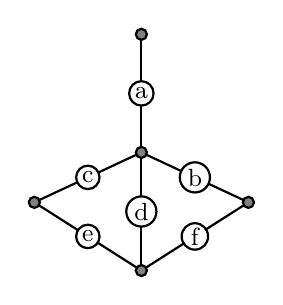
\begin{tikzpicture}[thick,scale=0.5]

	\coordinate (a1) at (90:3);
	\coordinate (a2) at (-25:3); 
	\coordinate (a3) at (-155:3);
	\coordinate (a4) at (-90:3);
	\coordinate (a5) at (0:0);

	\draw (a5)-- node [lblvertex] {a}(a1);
	\draw (a5)-- node [lblvertex] {b}(a2);
	\draw (a5)-- node [lblvertex] {c}(a3);
	\draw (a5)-- node [lblvertex] {d}(a4);
	\draw (a3)-- node [lblvertex] {e}(a4);
	\draw (a2)-- node [lblvertex] {f}(a4);

	\draw (a1) node {};
	\draw (a2) node {};
	\draw (a3) node {};
	\draw (a4) node {};
	\draw (a5) node {};
	%\draw (a1) node[lblvertex] {a};
	%\draw (a2) node[lblvertex] {b};  
	
\end{tikzpicture}
\pause\quad 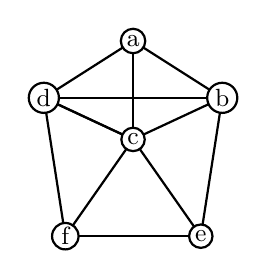
\begin{tikzpicture}[thick,scale=0.5]

	\coordinate (a) at (90:2.5);
	\coordinate (b) at (25:2.5); 
	\coordinate (c) at (0:0);
	\coordinate (d) at (155:2.5);
	\coordinate (e) at (-55:3);
	\coordinate (f) at (-125:3);

	\draw (a)--(b);
	\draw (b)--(c);
	\draw (c)--(d);
	\draw (d)--(a);
	\draw (a)--(c);
	\draw (c)--(d);
	\draw (b)--(e);
	\draw (e)--(c);
	\draw (d)--(f);
	\draw (f)--(c);
	\draw (d)--(b);
	\draw (e)--(f);
	%\draw (f) arc {-125:-33:3};
	
	\draw (a) node [lblvertex]{a};
	\draw (b) node [lblvertex]{b};
	\draw (c) node [lblvertex]{c};
	\draw (d) node [lblvertex]{d};
	\draw (e) node [lblvertex]{e};
	\draw (f) node [lblvertex]{f};
\end{tikzpicture}
\end{center}}
\bframe{Connected matching as a clique problem}{
	In the proximity coloring induced by $L(G)$
	\begin{itemize} 
		\uncover<2->{\item Blue edges correspond to a pair of incident edges in $G$} 
	 	\uncover<4->{\item Green edges correspond to a pair of disjoint edges in $G$ with some edge between them,} 
		\uncover<6->{\item Red edges correspond to separable edges.}
	\end{itemize}
	\begin{center}
		\uncover<3->{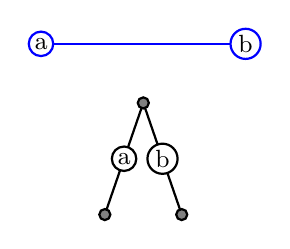
\begin{tikzpicture}[thick,scale=0.5]

	\coordinate (a0) at (0:0);
	\coordinate (a1) at (180:1);
	\coordinate (a3) at (-109:3);
	\coordinate (a2) at (0:1);
	\coordinate (a4) at (-71:3);
	\coordinate (b1) at (150:3);
	\coordinate (b2) at (30:3);

	\draw (a0)-- node[lblvertex] {a}(a3);
	\draw (a0)-- node[lblvertex] {b}(a4);
	\draw (b1)[blue]--(b2);
	\draw (a0) node {};	
	%\draw (a1) node {};
	%\draw (a2) node {};
	\draw (a3) node {};
	\draw (a4) node {};
	\draw (b1) node[lblvertex, draw = blue] {a};
	\draw (b2) node[lblvertex, draw = blue] {b};
\end{tikzpicture}
}\uncover<5->{\qquad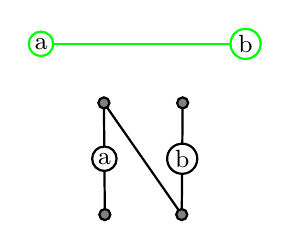
\begin{tikzpicture}[thick,scale=0.5]

	\coordinate (a0) at (0:0);
	\coordinate (a1) at (180:1);
	\coordinate (a3) at (-109:3);
	\coordinate (a2) at (0:1);
	\coordinate (a4) at (-71:3);
	\coordinate (b1) at (150:3);
	\coordinate (b2) at (30:3);

	\draw (a1)-- node[lblvertex] {a}(a3);
	\draw (a2)-- node[lblvertex] {b}(a4);
	\draw (a1)--(a4);
	\draw (b1)[green]--(b2);
	%\draw (a0) node {};	
	\draw (a1) node {};
	\draw (a2) node {};
	\draw (a3) node {};
	\draw (a4) node {};
	\draw (b1) node [lblvertex, draw = green]{a};
	\draw (b2) node [lblvertex, draw = green]{b};
\end{tikzpicture}
}\uncover<7->{\qquad\input{coresp3}}
	\end{center}\vskip 0.25 cm 
\uncover<8>{Connected matchings in $G$ then correspond to cliques in the green graph induced by $L(G)$.}}

\bframe{}{

We now restate our third partial result more precisely. \pause
\begin{theorem}
Let $c < 1/4$ be a constant.  For any constant $b$ and sufficently large $n$, every $\overline{K_3}$-free graph $G$ on $n$ vertices with $\omega(G) < b\sqrt{n\log n}$ has a $cn$-connected matching.
\label{sm_cli}
\end{theorem}
\pause\vskip 0.25 cm
The proof of this is simplest in the language of proximity colorings.  \pause\vskip 0.5 cm
We will show that (for large $n$) unless the clique number of $G$ is sufficiently large, the green graph induced by $L(G)$ has too many edges to avoid a $cn$ clique. 
}

\bframe{Proof}{

We will begin with a lemma phrased in terms of triangle free graphs.\pause
\blem{For every pair of positive constants $\epsilon, d$ there is $n_{\epsilon, d}$ such that every triangle-free graph $G$ with $n > n_{\epsilon, d}$ vertices and $\alpha(G) < d\sqrt{n\log n}$ has fewer than $\epsilon n^3$ induced copies of $C_4$.}\pause \vskip 0.5 cm
Note that induced copies of $C_4$ in the complement of a graph $G$ have a 1-1 correspondence to edges in the red graph induced by $L(G)$.
}

\bframe{Proof of Lemma}{

Fix $\epsilon, d> 0$ and let $G$ be a triangle free graph on $n$ vertices with $\alpha(G) < d\sqrt{n\log n}$. \pause \vskip 0.5 cm
Let $X_{C_4}$ be the number of $C_4$ in $G$. \pause \vskip 0.5 cm 
Then
\[X_{C_4} = \frac{1}{2}\sum_{\{u,v\}\notin E(G)} {|N(u) \cap N(v)| \choose 2}\]\pause
Set $\epsilon_1 < \sqrt{8\epsilon}$.
}

\bframe{Proof of Lemma, continued}{
\noindent Claim. \textit{For sufficiently large $n$, fewer than $n^2(\log n)^{-2}$ pairs of vertices $u,v$ have neighborhood intersection larger than $\epsilon_1\sqrt{n}$.}\pause \vskip 0.5 cm

Suppose the contrary is true, and there are more than $n^2(\log n)^{-2}$ pairs $u,v$ so that $|N(u)\cap N(v)| \geq \epsilon_1\sqrt{n}$. \pause \vskip 0.5 cm
When we count the total number of vertices in these intersections, the count is at least $\epsilon_1n^{5/2}(\log n)^{-2}$, meaning some vertex is counted at least $\epsilon_1n^{3/2}(\log n)^{-2}$ times. 
}

\bframe{Proof of Lemma, continued} {
However, $\Delta(G) \leq \alpha(G) < d\sqrt{n\log n}$, so each vertex is in at most \[{d\sqrt{n\log n}\choose 2 } < \frac{d^2}{2}n\log n\] neighborhood intersections.  Thus, for sufficiently large $n$,  the claim holds.
}

\bframe{Proof of Lemma, continued}{

Now we can bound $X_{C_4}$.\pause
\begin{eqnarray*}X_{C_4} <& \frac{1}{2}\left[\frac{n^2}{(\log n)^2}{d\sqrt{n\log n}\choose 2}+ \left( {n\choose 2}- \frac{n^2}{(\log n)^2}\right){\epsilon_1\sqrt{n}\choose 2}\right]\\\pause
\sim& \frac{\epsilon_1^2}{8}n^3 < \epsilon n^3
\end{eqnarray*}
Thus for sufficiently large $n$, $X_{C_4} < \epsilon n^3$.
}

\bframe{Proof of Theorem}{
\pause
Fix constants $d$ and $c < 1/4$, and let $G$ be a $\overline{K_3}$-free graph with $n$ vertices, $m$ edges, and $\omega(G) < b\sqrt{n\log n}$. \pause \vskip 0.5 cm
Consider the proximity coloring $\mathcal{P}$ induced by $L(G)$ (recalling that green $k$-cliques correspond to $k$-connected matchings in $G$ and red edges correspond to induced $C_4$s in $\overline{G}$). \pause \vskip 0.5 cm

We will apply T\'{u}ran's theorem to show that if $n$ is sufficiently large, then there are enough green edges to guarantee a green clique of size $cn$ in $\mathcal{P}$.

}

\bframe{Proof of Theorem, continued}{
 If $X_R, X_G,$ and $X_B$ denote the number of red, green and blue edges respectively, we would like to show that \[X_G = {m\choose 2} - X_R - X_B \geq {m\choose 2} - cn{m/cn\choose 2}\] \pause 
equivalently \pause
\begin{equation}
	X_R + X_B \leq cn{m/cn\choose 2}\label{goal}
\end{equation}
}

\bframe{Proof of Theorem, continued}{
We obtain a crude upper bound on $X_B$ by taking the number of edges in the line graph of $K_n$. \pause
\begin{equation}
	X_B < \frac{n^3}{2} - \frac{3n^2}{2} + n
\end{equation}\pause
We can also asymptotically bound $X_R$ using Lemma 1.  \pause For any $\epsilon > 0$ and sufficiently large $n$,\pause  \[X_B + X_R < \frac{n^3}{2} + \epsilon n^3\]
}

\bframe{Proof of Theorem, continued}{
We compare this with the right hand side of (\ref{goal})\pause
\begin{eqnarray}
	cn{m/cn\choose 2} =&\displaystyle \frac{cn}{2}\left(\frac{m^2}{c^2n^2} - \frac{m}{cn}\right)\\ \pause
	=& \displaystyle \frac{1}{2c}m^2n^{-1} - \frac{m}{2}\\ \pause
	\sim&   \displaystyle \frac{n^3}{8c}
\end{eqnarray}
Since $c < 1/4$, and we can take $\epsilon < \frac{1-4c}{8c}$, for sufficiently large $n$ (\ref{goal}) holds and $G$ has a $cn$-connected matching.
}


\section{Maximum Connected Matching}

\bframe{A computational problems}{
	Given an input graph we would like to be able to find a maximum connected matching.\pause
 	\begin{framed}
  		Maximum Connected Matching (MCM)
  		\vskip 0.25 cm Input: Graph $G$
  		\newline Output: Maximum connected matching of $G$
 	\end{framed}
	%We also may be interested in the largest connected portion of a given matching in $G$\pause
 	%\begin{framed}
  %		Maximum Connected Portion (MCP)
 % 		\vskip 0.25 cm Input: A matching $M$ from a graph $G$
 % 		\newline Output: Maximum connected portion of $M$
% 	\end{framed}
}

\bframe{Complexity results}{
	MCM is NP-hard in general for both the weighted and unweighted case \cite{MR2070161}. \pause\vskip 0.5 cm
	 Kathie Cameron has shown that MCM is NP-hard for 0-1 weighted bipartite graphs \cite{MR2163948}.\pause\vskip 0.5 cm
	 However, the problem is trivial for graphs with girth larger than 6 (hence, trees).\pause\vskip 0.5 cm
	Cameron also shows that MCM is polytime solvable on chordal graphs,.\pause \vskip 0.5 cm
 	We conjecture that MCM is polytime solvable on chordal bipartite graphs, and reduce this problem to the saturating problem on the same class.}
	 
\bframe{Chordal bipartite graphs}{
A graph in which every cycle of length six or greater has a chord is called {\it weakly chordal} or {\it weakly triangulated.}
\pause\vskip 0.5 cm
A weakly chordal graph that is also bipartite is called {\it chordal bipartite}.\pause\vskip 0.5 cm
\begin{center} 
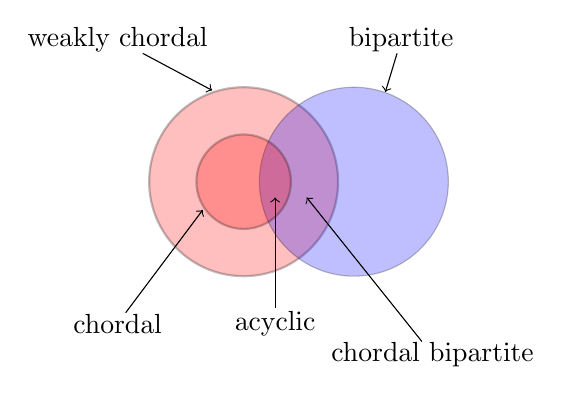
\begin{tikzpicture}[thick,scale=0.4]


\draw[ fill = red, opacity = 0.25] (0,0) circle (3);
\draw[ fill = blue, opacity = 0.25, thin] (3.5,0) circle (3);
\draw[ fill = red, opacity = 0.25] (0,0) circle (1.5);

\draw  (-4,4.5) node[words]{weakly chordal}
	edge [->, thin] (-1,2.9);

\draw  (-4,-4.5) node[words]{chordal}
	edge [->, thin] (-1.3,-0.9);

\draw (1,-4.5) node[words]{acyclic};
\draw node[words] (1,-4) {}
	edge [->, thin] (1,-.5);


\draw (6, -5.5) node[words]{chordal bipartite}
	edge[->, thin] (2,-.5);
\draw (5, 4.5) node[words]{bipartite}
	edge[->,thin] (4.5,2.85);

\end{tikzpicture}
 \end{center}
}

\bframe{A characterization of chordal bipartite graphs}{
A {\it bisimplicial edge} in a bipartite graph $G = (A, B; E)$ is an edge $uv$ with the property that for every neighbor $u'$ of $u$ and every neighbor $v'$ of $v$, the edge $u'$ and $v'$ is in E.\pause\vskip 0.5 cm
In other words, the neighborhoods of $u$ and $v$ induce a complete bipartite subgraph (a {\it biclique}).\pause\vskip 0.5 cm 
If we remove a bisimplicial edge from a chordal bipartite graph, the resulting graph is chordal bipartite.\pause\vskip 0.5 cm
Chordal bipartite graphs are precisely those that have a {\it bisimplicial elimination ordering}.  This is a sequence of edge removals so that each edge removed is bisimplicial and the result is an empty graph.
}
\bframe{An approach to MCM for chordal bipartite graphs}{
First, let us call an edge $e$ in $G$ {\it inert} if $\nu_c(G) = \nu_c(G-e)$. \pause\vskip 0.5 cm
\begin{prop}
Let $G = (A, B; E)$ be chordal bipartite.  A bisimplicial edge $e = uv$ is inert unless
	\begin{enumerate}
		\item $e$ is contained in every maximum connected matching.
		\item For any maximum connected matching $M$, every $f\neq e $ in $M$ has exactly one endpoint adjacent to $e$.
		\item  $N(e)$ is covered by $M$
	\end{enumerate}
\end{prop}


}

\bframe{Proof of 1}{
To show 1, we need to show that removing $e$ does not reduce the size of any maximum connected matching that does not include $e$.  \pause In fact this is true for any connected matching.\pause\vskip 0.5 cm
Suppose that $e = uv$ is bisimplicial. \pause Removing $e$ cannot disconnect edges $f_1$ and $f_2$.  \pause If $u$ is an endpoint of $f_1$ and $v$ is an endpoint of $f_2$, then the other endpoints of $f_1$ and $f_2$ must also be adjacent, owing to the bisimpliciallity of $e$.
}

\bframe{Proof of 2}{
Suppose now that $e$ and $f$ are in some maximum connected matching $M$, and both edges between the endpoints of $e$ and $f$ are present.  \pause\vskip 0.5 cm
We can replace $e$ and $f$ with these intermediary edges owing to the bisimpliciality of $e$.  
}

\bframe{Proof  of 3}{
If WLOG $u$ has a neighbor $v'$ not covered by $M$, then $e=uv$ can be replaced by $e'=uv'$
}

\bframe{Separable graphs}{A result of CITE shows that if $G$ is chordal bipartite and {\it separable}, then we can find two separable bisimplicial edges.  \pause\vskip 0.5 cm

If we have such a pair, it is clear from part 1 of the previous proposition that at least one is inert. \pause\vskip 0.5 cm

If we can efficiently determine which edge is inert, we can sequentially remove them until $G$ is no longer separable. \pause \vskip 0.5 cm

At this point we can apply a known maximum matching algorithm to obtain the maximum connected matching.
 }

\bframe{Reduction to a smaller problem}{

Suppose we have a separable pair $e = uv, f = xy$ of bisimplicial edges.\pause\vskip 0.5 cm
If $d(e) = d(f)$, then by part 1 of the previous proposition, both are inert and we can remove either one. \pause WLOG, assume $d(e) > d(f)$.  \pause \vskip 0.5 cm

Unless there is a connected matching between $N(u)$ and $\overline{N(v)}$ that saturates $N(u)$, and a connected matching between $N(v)$ and $\overline{N(u)}$ that saturates $N(v)$, then the previous proposition tells us $e$ is inert.\pause\vskip 0.5 cm

Otherwise, we have found a larger connected matching than any that contain $f$, and $f$ is therefore inert.

}

\bframe{Saturating connected matching (SCM)}{
Now we have a smaller problem. \pause
\begin{framed}
  		Saturating connected matching (SCM)
  		\vskip 0.25 cm Input: Bipartite graph $G = (A, B;E)$.
  		\newline Output: YES if there is a connected matching in $G$ covering $A$, NO otherwise.
 	\end{framed}\pause

If we can solve SCM in polynomial time for $G$ chordal bipartite, then we can solve MCM in polynomial time for $G$ chordal bipartite.
}

\bframe{A sufficient condition for SCM}{
 
Suppose $|A| =n$.  \pause If there is a sequence of distinct vertices $b_1, b_2, \ldots, b_n$ from $B$ and subsets $S_1, S_2, \ldots ,S_n$ of $A$ such that\pause
	\begin{enumerate} 
		\item $S_n = A$, \pause
		\item $S_i \subseteq S_j$ whenever $i < j$, \pause
		\item $S_k \subseteq N(b_k)$ for all $1 \leq k \leq n$, and\pause
		\item $|S_k| \geq k$ for all $1 \leq k \leq n$\pause
	\end{enumerate}
then there is a connected matching saturating $A$.
}

\bframe{Ordered connected matchings}{
A connected matching that has this property is called an {\it ordered } connected matching. PICTURE\pause\vskip 0.5 cm
Existence of this subgraph is equivalent to the condition as stated on the previous slide.
}

\bframe{A neccessary condition for SCM (chordal bipartite case)}{
In the chordal bipartite case, this condition is also neccessary.
\begin{prop}
	If $G$ is a chordal bipartite graph, then any connected matching $M$ in $G$ is ordered.
\end{prop}\pause\vskip 0.5 cm  
	We will show that a connected matching in a chordal bipartite graph has a vertex on each side that dominates the other side, and the ordering will follow.
}
\bframe{Proof}
{
 	We will proceed by induction on the size $n$ of the connected matching. \pause Small cases of $n = 1,2,3$ are obvious.  \pause \vskip 0.5 cm
	Assume now that the result holds for connected matchings up to $n-1$ edges, and let $M$ be a connected matching of $n$ edges in a chordal bipartite graph $G$.\pause \vskip 0.5 cm 

We will look at the subgraph $H$  induced by vertices covered by $M$.  \pause As we have observed previously, we can remove from $H$ any bisimplicial edges not contained in $M$ without reducing the size of $M$ \pause(or without introducing any new dominating vertices).  \pause  Remove such edges until any remaining bisimplicial edges are contained in $M$.
}

\bframe{Proof, cont.}{

The resulting graph is still chordal bipartite, so there exists a bisimplicial edge $xy$ contained in $M$. \pause If $y$ does not dominate $A$, look at the connected matching induced from $M$ by the neighbors of $x$ excluding $y$.  \pause \vskip 0.5 cm
Some $y'$ dominates the other side, which must contain all non-neighbors of $y$. \pause \vskip 0.5 cm The bisimpliciality of $xy$ ensures that $y'$ also dominates the neighbors of $y$.  \pause \vskip 0.5 cm Thus either $y$ or such a $y'$ dominates $A'$.  \pause (The argument can be repeated for $B'$ using $x$ instead of $y$.)  

}

\section{Future work}

\bframe{Where to go from here?}{

We have the following goals for the immediate future of this research:
\begin{itemize}\pause
	\item Improve partial result 3 of the extremal conjecture \pause
	\item Finish construction of a polytime algorithm for MCM on chordal bipartite graphs \pause
	\item Consider the complexity of weighted problem on chordal bipartite graphs, weighted and unweighted problems on weakly chordal graphs in general \pause
	\item Construct an efficient approximation algorithm for the general bipartite case 
\end{itemize}
}
\bframe{Thank you}{Questions?}

%\begin{bibsection}[Annotated Bibliography]\vspace{-\parskip} % This is the start of the bibliography. 
%	\begin{biblist}[\normalsize] % Replace the \bib entries with ones relevant to your problem.
							% The bulk of each entry can be copied and pasted from MathSciNet
							% ( http://www.ams.org/mathscinet/ ). When viewing the review of an
							% item you want to site, open the "Select alternative format" pull-down
							% and select AMSrefs.
							% Most likely, the only part you will need to change is the first parameter
							% after \bib. This is the internal name you use to cite the reference
							% with \cite. By default it will be the Mathematical Reviews number
							% (for example MR1375315). To make my life easier when I merge these all
							% into the summary document, please choose a name that begins with your
							% initials, followed by the number of problems you have submitted
							% (including this one).
							% For example, since this problem was submitted by Leonhard Euler and
							% since this is the first problem he is presenting, all citation names
							% begin with "le1". If this was his third problem, they would begin with
							% "le3".
%Z. Füredi, A. Gyárfás, G. Simonyi,  Connected matchings and Hadwiger's conjecture,  Combin. Probab. Comput., Problem Section, 14 (2005), 435--438.
%M. Kriesell, On seymour's strengthening of Hadwidger's conjecture for graphs with certain forbidden subgraphs 

%Mukhopadhyay, A. "The Square Root of a Graph." J. Combin. Th. 2, 290-295, 1967. 
\begin{thebibliography}{10}

\bib{MR671905}{article}{
   author={Duchet, P.},
   author={Meyniel, H.},
   title={On Hadwiger's number and the stability number},
   conference={
      title={Graph theory},
      address={Cambridge},
      date={1981},
   },
   book={
      series={North-Holland Math. Stud.},
      volume={62},
      publisher={North-Holland},
      place={Amsterdam},
   },
   date={1982},
   pages={71--73},
   review={\MR{671905 (84h:05074)}},
}

\bib{MR882610}{article}{
   author={Maffray, F.},
   author={Meyniel, H.},
   title={On a relationship between Hadwiger and stability numbers},
   journal={Discrete Math.},
   volume={64},
   date={1987},
   number={1},
   pages={39--42},
   issn={0012-365X},
   review={\MR{882610 (88g:05076)}},
   doi={10.1016/0012-365X(87)90238-X},
}


\bib{MR1411244}{article}{
   author={Toft, Bjarne},
   title={A survey of Hadwiger's conjecture},
   note={Surveys in graph theory (San Francisco, CA, 1995)},
   journal={Congr. Numer.},
   volume={115},
   date={1996},
   pages={249--283},
   issn={0384-9864},
   review={\MR{1411244 (97i:05048)}},
}
\bib{MR1654153}{article}{
   author={Reed, Bruce},
   author={Seymour, Paul},
   title={Fractional colouring and Hadwiger's conjecture},
   journal={J. Combin. Theory Ser. B},
   volume={74},
   date={1998},
   number={2},
   pages={147--152},
   issn={0095-8956},
   review={\MR{1654153 (99k:05079)}},
   doi={10.1006/jctb.1998.1835},
}
\bib{MR1844036}{article}{
   author={Kotlov, Andre{\u\i}},
   title={Matchings and Hadwiger's conjecture},
   note={Algebraic and topological methods in graph theory (Lake Bled,
   1999)},
   journal={Discrete Math.},
   volume={244},
   date={2002},
   number={1-3},
   pages={241--252},
   issn={0012-365X},
   review={\MR{1844036 (2002k:05087)}},
   doi={10.1016/S0012-365X(01)00087-5},
}



\bib{MR2163948}{article}{
   author={Cameron, Kathie},
   title={Connected matchings},
   conference={
      title={Combinatorial optimization---Eureka, you shrink!},
   },
   book={
      series={Lecture Notes in Comput. Sci.},
      volume={2570},
      publisher={Springer},
      place={Berlin},
   },
   date={2003},
   pages={34--38},
   review={\MR{2163948 (2006c:90072)}},
   %doi={10.1007/3-540-36478-1_5},
}

\bib{MR1979786}{article}{
   author={Klazar, Martin},
   title={Non-$P$-recursiveness of numbers of matchings or linear chord
   diagrams with many crossings},
   note={Formal power series and algebraic combinatorics (Scottsdale, AZ,
   2001)},
   journal={Adv. in Appl. Math.},
   volume={30},
   date={2003},
   number={1-2},
   pages={126--136},
   issn={0196-8858},
   review={\MR{1979786 (2004h:05006)}},
   doi={10.1016/S0196-8858(02)00528-6},
}



\bib{MR2070161}{article}{
   author={Plummer, Michael D.},
   author={Stiebitz, Michael},
   author={Toft, Bjarne},
   title={On a special case of Hadwiger's conjecture},
   journal={Discuss. Math. Graph Theory},
   volume={23},
   date={2003},
   number={2},
   pages={333--363},
   issn={1234-3099},
   review={\MR{2070161 (2005e:05055)}},
}

\bib{FGS}{article}{
   author={F\"{u}redi, Zolt\'{a}n},
   author={Gy{\'a}rf{\'a}s, Andr{\'a}s},
   author={Simonyi, G\'{a}bor}
   title={Connected matchings and Hadwiger's conjecture},
   journal={Combin. Probab. Comput.},
   part={Problem Section},
   volume={14},
   date={2005},
   pages={435--438},
}


\bib{MR2156345}{article}{
   author={Kawarabayashi, Ken-ichi},
   author={Plummer, Michael D.},
   author={Toft, Bjarne},
   title={Improvements of the theorem of Duchet and Meyniel on Hadwiger's
   conjecture},
   journal={J. Combin. Theory Ser. B},
   volume={95},
   date={2005},
   number={1},
   pages={152--167},
   issn={0095-8956},
   review={\MR{2156345 (2006b:05118)}},
   doi={10.1016/j.jctb.2005.04.001},
}


\bib{MR2249267}{article}{
   author={Gy{\'a}rf{\'a}s, Andr{\'a}s},
   author={Ruszink{\'o}, Mikl{\'o}s},
   author={S{\'a}rk{\"o}zy, G{\'a}bor N.},
   author={Szemer{\'e}di, Endre},
   title={One-sided coverings of colored complete bipartite graphs},
   conference={
      title={Topics in discrete mathematics},
   },
   book={
      series={Algorithms Combin.},
      volume={26},
      publisher={Springer},
      place={Berlin},
   },
   date={2006},
   pages={133--144},
   review={\MR{2249267 (2008c:05120)}},
   %doi={10.1007/3-540-33700-8_8},
}

\bib{FGS}{article}{
   author={Kriesell, Matthias},
   title={On Seymour's strengthening of Hadwiger's conjecture for graphs with certain forbidden subgraphs},
   journal={Discrete Mathematics},
   %volume={},
   date={2010},
   pages={435--438},
}

\bib{MR0297600}{article}{
   author={Chv{\'a}tal, V.},
   author={Erd{\H{o}}s, P.},
   title={A note on Hamiltonian circuits},
   journal={Discrete Math.},
   volume={2},
   date={1972},
   pages={111--113},
   issn={0012-365X},
   review={\MR{0297600 (45 \#6654)}},
}

\bib{MR1369063}{article}{
   author={Kim, Jeong Han},
   title={The Ramsey number $R(3,t)$ has order of magnitude $t\sp 2/\log t$},
   journal={Random Structures Algorithms},
   volume={7},
   date={1995},
   number={3},
   pages={173--207},
   issn={1042-9832},
   review={\MR{1369063 (96m:05140)}},
   doi={10.1002/rsa.3240070302},
}

\bib{MR0284366}{article}{
   author={Nash-Williams, C. St. J. A.},
   title={Edge-disjoint Hamiltonian circuits in graphs with vertices of
   large valency},
   conference={
      title={Studies in Pure Mathematics (Presented to Richard Rado)},
   },
   book={
      publisher={Academic Press},
      place={London},
   },
   date={1971},
   pages={157--183},
   review={\MR{0284366 (44 \#1594)}},
}

\bib{edhc}{article}{
	author={Christofides, Demetres},
	author={K\"{u}hn, Daniela},
	author={Osthus, Deryk},
	title={Edge-disjoint Hamilton cycles in graphs},
	date={31 Aug 2009},
	eprint={arXiv:0908.4572v1 [math.CO]},
	url={http://arxiv.org/abs/0908.4572},
}

\bib{MR1851303}{book}{
   author={Vazirani, Vijay V.},
   title={Approximation algorithms},
   publisher={Springer-Verlag},
   place={Berlin},
   date={2001},
   pages={xx+378},
   isbn={3-540-65367-8},
   review={\MR{1851303 (2002h:68001)}},
}

\end{thebibliography}
\nocite{*}
\end{document}
